\documentclass[12pt,letterpaper]{article}

\usepackage{graphicx,
			amssymb,
			amsmath,
			titlesec,
			lipsum,
			setspace,
			lastpage,
			fancyhdr,
			tikz,
			titling}
\usepackage{tkz-euclide}
\usepackage{setspace}
\usepackage{hyperref}

\usetkzobj{all}
\usetikzlibrary{shapes,arrows}
\tikzstyle{block} = [rectangle, draw, fill=blue!20,
text centered, rounded corners, minimum height=2em]

\tikzstyle{line} = [draw, -latex']
\newenvironment{my_enumerate}{
	\begin{enumerate}
	\setlength{\itemsep}{1pt}
	\setlength{\parskip}{0pt}
	\setlength{\parsep}{0pt}}{\end{enumerate}
}

%% Figure caption formatting
\usepackage[labelfont=it,textfont=it,labelsep=period]{caption}
\usepackage[labelfont=it,textfont=it,labelsep=period]{subcaption}

%% Overall margins
\usepackage[margin=1in]{geometry}

%% Footer formatting
\fancyhf{}
\renewcommand{\headrulewidth}{0pt}
\pagestyle{fancy}
\cfoot{\textbf{\textsf{Page\ \thepage\ of \pageref{LastPage}}}}

%% Author list formatting
\newenvironment{nscenter}
 {\parskip=0pt\par\nopagebreak\centering}
 {\par\noindent\ignorespacesafterend}

\newcommand{\affiliatedauthor}[2]{
\begin{nscenter}
	#1 \\ \textit{#2}
\end{nscenter}
}

%% Abstract formatting
\renewcommand{\abstractname}{ABSTRACT}

\renewenvironment{abstract}
 {\vspace{-0.5ex}
	\small
	\begin{center}
		\bfseries \abstractname\vspace{-4ex}\vspace{0pt}
	\end{center}
	\list{}{
		\setlength{\leftmargin}{0.5in}
		\setlength{\rightmargin}{\leftmargin}
	}
	\item\relax}
 {\endlist}

%% Section header formatting
\renewcommand\thesection{}
\renewcommand\thesubsection{}
\renewcommand\thesubsubsection{}
\titleformat{\section}{\normalfont\bfseries}{\thesection}{1em}{}
\titleformat{\subsection}{\normalfont\bfseries}{\thesubsection}{1em}{}
\titleformat{\subsubsection}{\normalfont\itshape}{\thesubsubsection}{1em}{}
\titlespacing*{\section}{0pt}{2ex}{-1.5ex}
\titlespacing*{\subsection}{0pt}{2ex}{-1.5ex}
\titlespacing*{\subsubsection}{0pt}{2ex}{-1.5ex}

%% Paragraph formatting (changing this messes with literally everything)
\setlength{\parindent}{0pt}
\setlength{\parskip}{2ex}
\newcommand\tab[1][1cm]{\hspace*{#1}}

\title{Humanized Quadcopter Swarm System for IARC 2019}

\begin{document}

\begin{center}
	\textbf{\LARGE{\thetitle}}
\end{center}

%%%%%%%%%%%% SET AUTHOR NAMES AND AFFILIATIONS %%%%%%%%%%%%
\affiliatedauthor{Umer Salman, Noel Brownback, Eric Johnson, Mario Gonzalez}{The University of Texas at Austin}
%%%%%%%%%%%%%%%%%%%%%%%%%%%%%%%%%%%%%%%%%%%%%%%%%%%%%%%%%%%


%%%%%%%%%%%%%%%%%%%%%%% ABSTRACT %%%%%%%%%%%%%%%%%%%%%%%
\begin{abstract}
	Texas Aerial Robotics has constructed a custom quadrotor aircraft system for the fulfillment of the International Aerial Robotics Competition Mission 8. A combination of lightweight materials and powerful propulsion optimizes flight time, while standardized flight control systems supported by a massive community enables customization and adaptation to the mission at hand. This includes the integration of a multitude of sensors that enhance environmental awareness and allow for the aiding of people to analyze and interact with an environment. This is done through homebrewed QR code decoding algorithms and the shared computing power onboard the multiple aircrafts. Safe development has been assured by strategic selection of components, thorough vetting of software in Software in the Loop simulation, and robust testing procedures in secure areas.
\end{abstract}
%%%%%%%%%%%%%%%%%%%%%%%%%%%%%%%%%%%%%%%%%%%%%%%%%%%%%%%%

%%%%%%%%%%%%%%%%%%%%%% MAIN TEXT %%%%%%%%%%%%%%%%%%%%%%

\section*{INTRODUCTION}
	Previous aerial robotics missions have always allowed for GPS or other external active position estimation that allowed for constant locational awareness. Location data is important to any mission, as proper state awareness prevents various failures, including complete loss of control for the drone. Thus, Mission 8 requires novel solutions to deriving this critical state data as GPS is forbidden. Additionally, the aircrafts must be capable of taking commands in a humanized ``natural'' fashion and avoid other aircrafts without being informed of those other aircrafts' locations.

	Texas Aerial Robotics addresses these challenges by utilizing computer vision. TAR uses ORBSLAM2, an ``Open-Source SLAM System for Monocular, Stereo and RGB-D Cameras'' to create maps of the arena in real time. The drone creates pointclouds of the objects in view using the stereo camera and combines sections together to create the maps. This means that should a section of the map start showing drift, the ORBSLAM2/ORBSLAMM System will toss out just the section while maintaining as much of the map as possible. TAR hopes to combine the processing between the multiple drones to have them work together on one map. These drones also solve for the QR code that is the combination the human needs for collecting the objects. TAR implements the ``humanized'' control aspect of the system through voice control using an Android app that connects to all of the air vehicles. The drones are also built with safety features for a plethora of other objects that may be on the field through its man-safe propellers for any humans and sonar sensors for avoiding other air vehicles at all times.

	One important aspect of TAR’s system is that it is very modular and interchangeable. Drone A is meant to be identical to Drone B and each drone can operate as any other. This creates a more robust drone swarm as the mission is still doable with as few or as many drones and no one drone is the hinge that the entire system needs to function.

	\begin{figure}[!htbp]
		\begin{center}
			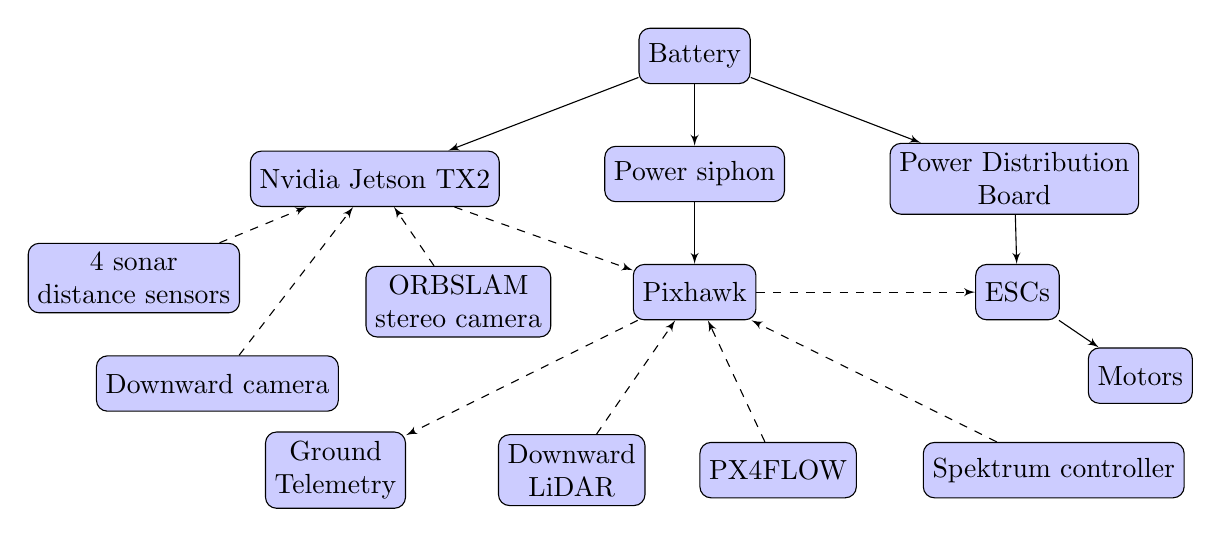
\begin{tikzpicture}[node distance = 1.5cm and 8cm, auto]
				\node [block] (battery) {Battery};
				\node [block, below of=battery] (siphon) {Power siphon};
				\node [block, below of=siphon] (Pixhawk) {Pixhawk};
				\node [block, below right of=battery, xshift=3cm, yshift=-.5cm, align=center] (PDB) {Power Distribution \\ Board};
				\node [block, below left of=battery, xshift=-3cm, yshift=-.5cm] (Jetson) {Nvidia Jetson TX2};
				\node [block, right of=Pixhawk, xshift=2.6cm] (ESCs) {ESCs};
				\node [block, below right of=ESCs, xshift=.5cm] (Motors) {Motors};
				\node [block, below right of=Jetson, yshift=-.5cm, align=center] (StereoCamera) {ORBSLAM \\ stereo camera};
				\node [block, below of=Jetson, xshift=-2cm, yshift=-1.1cm, align=center] (DownCamera) {Downward camera};
				\node [block, xshift=-2cm, yshift=-.2cm, below left of=Jetson, align=center] (Sonars) {4 sonar \\ distance sensors};
				\node [block, below right of=Pixhawk, yshift=-1.2cm] (Flow) {PX4FLOW};
				\node [block, below right of=Pixhawk, xshift=3.5cm, yshift=-1.2cm] (Spektrum) {Spektrum controller};
				\node [block, below left of=Pixhawk, xshift=-.5cm, yshift=-1.2cm, align=center] (LiDAR) {Downward \\ LiDAR};
				\node [block, below left of=Pixhawk, xshift=-3.5cm, yshift=-1.2cm, align=center] (Telemetry) {Ground \\ Telemetry};
				% Draw edges
				\path [line] (battery) -- (siphon);
				\path [line] (siphon) -- (Pixhawk);
				\path [line] (battery) -- (PDB);
				\path [line] (PDB) -- (ESCs);
				\path [line] (battery) -- (Jetson);
				\path [line, dashed] (StereoCamera) -- (Jetson);
				\path [line, dashed] (DownCamera) -- (Jetson);
				\path [line, dashed] (Sonars) -- (Jetson);
				\path [line, dashed] (Flow) -- (Pixhawk);
				\path [line, dashed] (Jetson) -- (Pixhawk);
				\path [line, dashed] (LiDAR) -- (Pixhawk);
				\path [line, dashed] (Pixhawk) -- (Telemetry);
				\path [line, dashed] (Spektrum) -- (Pixhawk);
				\path [line, dashed] (Pixhawk) -- (ESCs);
				\path [line] (ESCs) -- (Motors);
			\end{tikzpicture}
		\caption*{Flowchart of quadcopter electronics \\ \scriptsize *Solid arrows indicate power while dashed lines indicate power+data}
		\end{center}
	\end{figure}

	\pagebreak
	\subsection*{Texas Aerial Robotics Yearly Milestones}

	\begin{itemize}
		\item 2017 (Mission 7) - Have a working bot, with computer vision software in nearly working state for IARC Mission 7, a Roomba herding challenge.

		\item 2018 (Mission 7) - Continue development of computer vision, develop a computational game strategy through creation of simulations of the motion of Roombas, and tweak the physique of the drone for better flight control and stability.

		\item 2019 (Mission 8) - Complete a working system, with localization and GPS-denied navigation of multiple drones. These drones should work together to solve the QR code and communicate with a person through an Android app that can transmit voice commands to the drones.

		\item 2020 (Mission 8) - Finish all aspects of mission through more networking and collaboration between the quadcopters, improve the drone for better flight control and overall size, have better communication between drones to know where enemy drones are at all times, add aesthetic design choices, and test for hours in gyms in as many conditions as possible.
	\end{itemize}

\section*{AIR VEHICLE}
	\subsection*{Propulsion and Lift System}
	The vehicle utilizes an y axis symmetrical quad-rotor system. This H-frame provides a stable quadcopter for a smaller overall package while maintaining plenty of room for electronics. The frame is lifted by four T-Motor MN2212 KV920-V2.0 motors. These motors provide 0.92 [kg] of thrust per motor at 100\% throttle when paired with a 4-cell battery and 9.5 [in] propellers for total 3.68 [kg] of thrust. This is necessary for our 1.95 [kg] weight to maintain a thrust-to-weight ratio of 1.88, for battery life and flight time.

	The propellers used with the motors are 9.5 [in] long and made of plastic. These T-Motor propellers provide excellent precision, durability, and efficiency. The rotors are placed to counter-rotate for flight stability and to retain a one-to-one ratio of propellers to motors.

	\subsection*{Power Management System}
	The quadcopter uses a 4000 [mAh] 4S 25C LiPo battery for power. With 4 T-Motor MN2212 KV920-V2.0 motors running at close to 60\% throttle, a 4 Cell battery was necessary to reach the 480 [grams] of thrust per motor needed for hovering flight.
	\begin{center}
		$T_{min} = \frac{\text{Battery power}(AH) * 60}{\text{Total current drawn by motors}}$
	\end{center}

	Assuming an average throttle of 65\% for maneuvering, we see a 4 A current draw from each motor, and with a 4000 mAh battery, that provides us with 13 minutes of flight time with minimal maneuvering and height change. This gives us plenty of headroom for more intense altitude and positioning changes, which will allow us to move more quickly during the competition, a valuable asset with the given time limitation.
	\begin{center}
		Max continuous Amp draw ($A$) = Battery capacity ($Ah$) $*$ Discharge rate ($C$)
	\end{center}

	To save on weight and space, we chose a 25C discharge rate battery, as this is still more than enough to match the maximum continuous current draw of 100 [A] and maximum practical current draw of 29.6 [A] required by the motors. The Pixhawk flight controller and Jetson TX2 compute unit will be powered of the same 4000 [mAh] battery. Together, they contribute a maximum practical current draw of 2.2 [A]. The 4000 [mAh] battery with a 25C discharge rate gives us a maximum continuous current draw of 100 [A], well exceeding the limit of the motors and computing units combined.

	The eCalc online tool was used to validate our calculations, and as seen by the graph on the following page, there should be no issue reaching flight times of 8 minutes at speeds below 15 [mph].

		\begin{figure}[!htbp]
			\begin{center}
				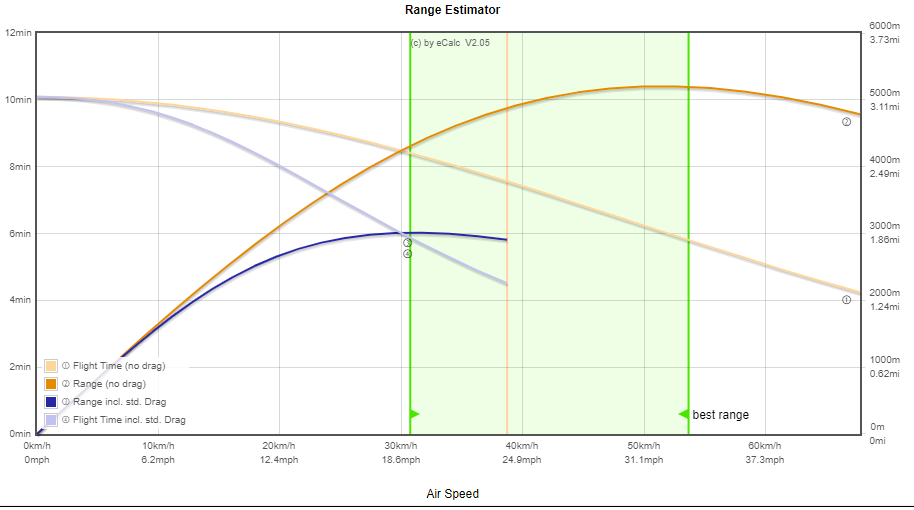
\includegraphics[width=\textwidth]{powerGraph}
			\end{center}
		\end{figure}

\pagebreak

	\subsection*{Flight Control System}
		\subsubsection*{Navigation/State Estimation System}

		Our system builds off of the robust open source project ArduCopter. ArduCopter, which runs on the Pixhawk, controls the stability and position control of the drone by taking in data from the IMU, compass, altitude ToF, and a position estimate generated from our optical flow sensor or ORB SLAM. The ArduCopter flight stack is maintained by hundreds of developers from around the world and the software is deployed on thousands of commercial and recreational drones. The vast community of developers and users ensures reliable controls code with lots of features.

		We have made slight modifications to the ArduCopter firmware, which allow us to set the EKF origin from our GNC ROS node. This has been done to make our drones capable of navigating in GPS denied environments. For general waypoint navigation, the drones utilize the ArduCopter EKF that takes in data from the sensors listed above, including the optical flow, compass, and IMU. The EKF position is then queried via mavros so that our navigation code can use our position to make intelligent decisions. TAR has greatly improved ArduCopter’s GPS denied capabilities by integrating ORBSLAM into the ArduCopter EKF. The use of ORBSLAM allows the drone to navigate based on 3 dimensional visual features in the drones operating environment. ORBSLAM continuously builds a map of its environment and compares current local maps to its master. Because of this comparison algorithm, ORBSLAM is able to perform loop closure, which is useful in negating any propagated error from the rate sensors.

		In addition to the stability and position control from ArduCopter, TAR’s drone sports a navigation node, which executes our pathplaning algorithms developed for Mission 8. The navigation node determines a waypoint and mode, then does a sanity check on the waypoint before publishing the waypoint to ArduCopter until the drone has reached its destination.

		\subsubsection*{Attitude/Position Control System}

		A crucial aspect of navigating in a GPS-denied area is concrete information on our position. Using a Teraranger One Time of Flight sensor from Terabee, our drones are able to know their exact altitude. This sensor was chosen due to its extremely light weight over other LiDAR options. This communicates over I2C directly to the Pixhawk where ArduCopter uses that information in the EKF.

		The position control aspect is handled through ORBSLAM running on the Jetson which is then fed into ArduCopter on the Pixhawk. The stereo camera in the front of the aircraft allows visual and depth information of the objects on the field. This information is used to formulate an estimate of the drone’s position based on the 3 dimensional visual features of the environment. In addition, these features are compared to features the drone has already seen in order to perform loop closure. Loop closure is then used to correct for propagated error accumulated from the drone’s rate sensors. No sensor or algorithm is foolproof. ORBSLAM has some limitations which limit the algorithms ability to generate position estimates. First, if the camera is moved too quickly, the deltas between frames is too large and ORBSLAM can lose tracking. This is mostly mitigated by limiting the drones flight velocity. The second limitation of ORBSLAM is the requirement of textures and 3D features. Both of these risks are low when operating in the Mission 8 arena, however, this is a flight critical system and the consequence of failure are catastrophic. TAR has opted to implement redundancy by attaching the PX4FLOW sensor to supplement ORBSLAM in the event of failure. While not as useful on the non-textured surface, it should at least ensure that the drone does not lose control.

		The quadcopter uses eight sensors for flight control. The main sensors used for the navigation of the quadcopter include a downward-facing 1D LiDAR module, a PX4FLOW optical sensor, and the built-in sensors of the Pixhawk 2 flight control board.

		The 1D LiDAR module used is a Time of Flight (ToF) sensor named the Teraranger One. This one-dimensional sensor is directed downward and provides data to determine altitude. The PX4FLOW sensor measures velocity by comparing frame by frame images and measuring the distance traveled and direction. As previously stated this sensor is a redundancy for ORBSLAM. The Pixhawk 2 contains three 3-axis accelerometers, three 3-axis gyroscopes, and two 3-axis compasses. The data from these sensors is used by the Pixhawk onboard system for flight control and maneuvering of the quadcopter.

		\begin{figure}[!htbp]
			\begin{center}
				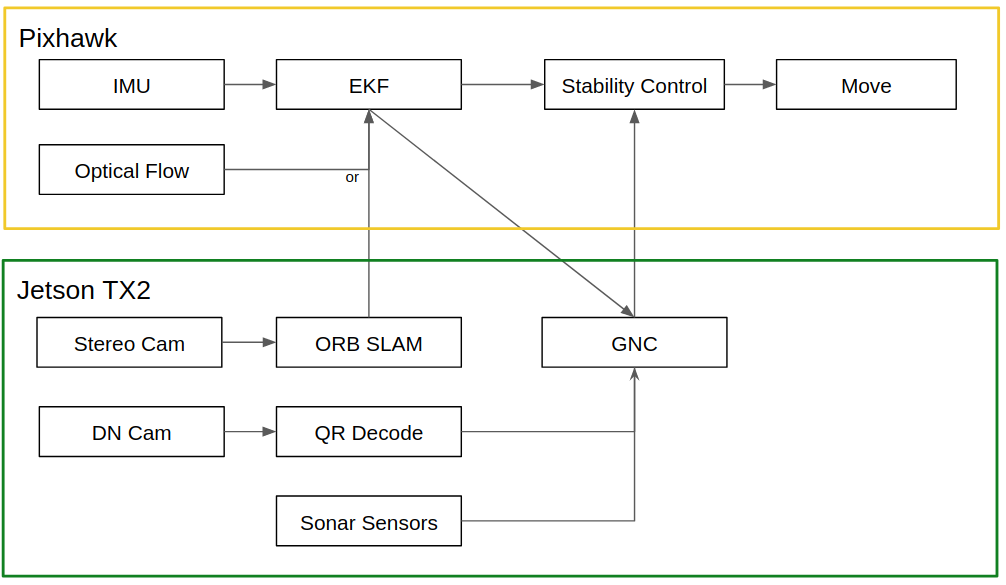
\includegraphics[width=0.75\textwidth]{system}
				\caption*{Overview of control system}
			\end{center}
		\end{figure}

		\subsubsection*{Flight Termination System}
		We will be using ArduCopter's EmergencyStop to act as our killswitch. In the event of catastrophic failure, the safety operator can send the kill signal, and all power will immediately be cut from the drone's ESCs, and in turn, the motors.


\section*{MISSION PACKAGE}
	The drone has been designed to carry all the necessary GNC sensors, an array of sonar sensors, a stereo camera, a downward camera, and a Nvidia Jetson TX2. In addition, the drone carries a telemetry radio, WiFi antennas, and an RC receiver in order to carry out safe flight.
	\subsection*{Perception System}
	For completion of Mission 8, the drone must be able to detect the QR code and avoid obstacles, both moving and non-moving. The quadcopter is equipped with a single downward facing camera for reading the quadrant of the QR code. A stereo camera is used for ORBSLAMM for localization. There is also an array of sonar sensors for obstacle avoidance.

		\subsubsection*{Target Identification and Behavior}
		For target identification and behavior, the drones fly to defined waypoints where the quadrants of the QR codes are located. Each quadcopter is equipped with a singular ELP webcam facing downward. This camera was chosen for its very light weight while still allowing adjustment of exposure and other parameters to better read a QR code on an iPad.

		Once the QR code quadrant is in view, computer vision begins to process using our algorithm that uses the inherent features of QR codes. Any drone is able to narrow down the 4 digit combination to approximately 6 permutations that from only the bottom-right quadrant. The drones continue to scan the other sections of the QR code and piece together the combination. If the top-right quadrant is found, then the code is complete with only the top-right and bottom-right sections.

		After the code has been identified, the quadcopters fly to positions on the field where the human would likely choose to heal and await other commands.

		\subsubsection*{Threat Identification and Behavior}
		Our avoidance system takes data from an array of sonar sensors. These 4 MAXBOTICS 7m I2C sonars allow the drone to detect objects on the sides the quadcopter intends to move in. This data is passed to the navigation node, which uses this data to determine if an obstacle drone or a wall is within 1.5 [m], in which case the node will issue a waypoint opposite the detections. Edge cases and corner cases have also been accounted for, such as the case where an enemy drone pushes a helper drone against a wall. In this case, the drone will either rise or fall in altitude, depending on the distance from the ground. Each drone has its own array of sonar sensors, so even in the event of communication failures between quadcopters in the full system, each drone will continue to intelligently avoid dangerous situations.

		Sonar sensors were chosen for obstacle detection rather than a 2D LiDAR or webcams to save on weight, space, and computing power. Sonar sensors are very tried and true. As we use I2C as our communication protocol for these sonars, adding or subtracting sensors to the array becomes trivial, with easy addition of more sonar sensors (up to a limit of 127) with very few modifications to the code, electrical systems, and/or hardware, aside from the physical mounting of the new sonars themselves. Additionally, sonar was picked over radar as radar has a harder time picking up smaller objects, like a drone.

		Other threat identification systems, such as an infrared cameras, were discussed. However, potential interference from sunlight and other environmental factors led the team to choosing sonars instead.

		\subsubsection*{Gesture Identification and Behavior}
		For the humanized controls, TAR opted not to go for gesture recognition as gesture recognition poses many challenges regarding identifying which drone is being commanded and the characteristics of the person, such as height and size. Additionally, the person needs to get the QR code information from the drones. For this TAR developed an Android app. Once we had the Android app, it became clear that voice recognition made more sense for commanding the air vehicles. The voice recognition is done on the Android device and the information is sent over the 2.4 GHz WiFi network to the drone that is being commanded. The details of this app is defined in the Man/Machine Interface subsection below.

	\subsection*{Communications Systems}
	On each Jetson, data is passed between software nodes via ROS. Commands to the flight computer from that Jetson are passed via serial connection with data encoded in MAVLINK messages. Data between our multiple Jetsons (1 per drone) is passed via ROS messages through a 2.4 GHz WiFi network. The quadcopters connect to Texas Aerial Robotics’ router, which maps the quadcopters to IP addresses. The drones are interchangeable on the network-side too as the drones to IP addresses is not hard defined, resulting in a more modular and more robust system.

	\subsection*{Man/Machine Interface}
	The drone has a DX7 RC controller interface for system checks and emergency situations. In addition, the flight controller can be monitored via a telemetry radio using Mission Planner. Our autonomous scripts must be initiated by an SSH connection to our Nvidia Jetsons.

	A crucial part of the Man/Machine Interface is the Android app that handles humanized communication to and from the air vehicles. Texas Aerial Robotics was able to spin this up quickly by using the same method of building off open-source projects. For this Android application, we built off ROSJava (running on the Android phone) to be able to open ROS Subscribers and Publishers on a remote device (the drones). The drones can publish to the Android phone once they have completed the QR code and the Android phone displays the data. Additionally, this Android app also handles the voice recognition aspect. Using the open-source project PocketSphinx from Carnegie Mellon University, TAR was able to implement on device voice recognition with a custom command dictionary. This was developed in a seperate app until ready. Then the two apps were combined to give one view for communicating to and from the drones over ROS from that Android device. TAR will use headphones with a clip-on microphone for listening to the person so the voice is clear. This app was developed with the ability to use it on Android Wear as well, so a user could just as easily use a smartwatch as the interface device for commanding the drones.


\section*{OPERATIONS}
	\subsection*{Flight Preparations}
		\subsubsection*{Checklist}
			\begin{my_enumerate}
				\item Check battery voltage and insert
				\item Make sure LiDAR, PX4FLOW, and cameras are not covered
				\item Make sure that the props are on in the correct direction (leading edge in)
				\item Make sure prop guards are secure
				\item Make sure Kill Switch is in correct position
				\item Power on controllers
				\item Make sure ground station has good telemetry
				\item Verify critical sensors are giving good data
				\item Plug in TELEM2
				\item SSH start/verify autonomous scripts are running
				\item Make sure everyone is clear of drone
				\item Verify mode switch in Stabilize
				\item Hold safety button
				\item Mode switch to Autonomous
			\end{my_enumerate}

\section*{RISK REDUCTION}
	\subsection*{Vehicle Design}
		\subsubsection*{EMI/RFI Solutions}
			The Arducopter flight stack helps keep interference risk down through the EMI motor calibration on the Pixhawk. The calibration calculates the magnetic interference correction by formulating a function of the magnetic interference based on the power setting of the motors. Additionally, the drone was designed to reduce the electromagnetic interference in the first place through the use of carbon fiber over the high voltage electronics. Antennas and other radio connections are then done above the carbon fiber.

		\subsubsection*{Shock/Vibration Isolation}
			The modern Pixhawk flight controller contains internal damping from the vibration of the drone's structure. The team decided that there is no need for extra damping. After completion of our drones, flight logs from the Pixhawk confirmed that vibration on the quadcopter was well within recommended amounts. The team believes there is no need to have landing legs or landing shocks. In flight, the drone stays stable and the sensors give good readings throughout the 20 minutes of flight time each drone can get. Because of this, TAR believes no inflight shocks or vibrations will interfere with the guidance or navigation of the drone.


	\subsection*{Safety}
		We took significant steps to ensure safe operation of the quadcopter. In order to keep the quadcopter from flying where we do not want, we have a Spektrum receiver module onboard so our designated safety pilot can manually control the vehicle. Additionally, we are able to check the status of the quadcopter through our telemetry to our ground station.

		An important part of IARC Mission 8 is the Human in the Loop. Safety is dialed up to 11 when a person is near the quadcopters. For this, each drone is outfitted with propeller guards to mitigate damage to people or property. We wanted a design that would interfere with the prop wash as little as possible, but still be able to prevent a human from accidentally sticking a finger in the path of the blades. These prop guards protect the drone from damage, but more importantly, the human from damage. These prop guards are also easily removable, should a situation arise where the quadcopter not need the guards or parts need to be quickly replaced.

		Also an important safety feature is the sonar sensor array discussed earlier. This important feature keeps each drone from getting close to anything in flight in the first place.

		The last important safety feature is the kill switch. The kill switch is one developed by the ArduCopter team. Should the kill command be sent, the Pixhawk shuts off the ESCs immediately. This has been a feature of ArduCopter for multiple software versions and has been tested all around the world. Because of its testing through being in ArduCopter, it is a far more tried and true method than one TAR could implement otherwise.


	\subsection*{Modeling and Simulation}
	For Mission 8, the computational team developed a simulation of Mission 8 with Gazebo and ROS software. With this simulation, TAR was able to perform software in the loop simulation and conduct mission planning without jeopardizing the physical drone.

	The simulation was first constructed by building models according to the specifications provided by IARC. The models were built in Solidworks and edited with Blender software to texture the models and export as COLLADA files. With these COLLADA files, the properly textured models were loaded into the Gazebo simulation. The models constructed consisted of the arena, the bunkers, the bins, and the QR codes. Moreover, a controllable human was inserted into the simulation. To simulate the helper drone(s), TAR imported a standard quadcopter model from the ArduCopter standard library, similar to what was done for Mission 7. On the drone model, TAR added the same sensors used on the physical drone such as stereo cameras and sonar. With this model, all the software components of the drone such as the flight code and ORBSLAM2 could be tested.

	Going into more detail, the human model was made controllable with C++ scripts that utilized ROS software to input movement commands. Likewise, the drone was controlled through ArduCopter and ROS and demonstrated the desired autonomous behavior that was to be congruent with the actual physical drone’s behavior. Also, for added robustness, the QR codes within the arena could be randomly changed through a simple bash script; this allowed us to quickly test our QR code reading with different QR code combinations.

	Lastly, with hardware generously donated to us by Emergent Space Technologies, Virtual Reality (VR) was implemented into the human model for mission planning and demonstration. We added a camera to the human model’s head and exported the feed to the VR headset to simulate what it would actually be like to be inside the arena. With this perspective, the team had a unique insight into the conditions of the arena that would be otherwise unobtainable without physical access to the actual arena.

	With this simulation, Texas Aerial Robotics is able to test drone software and perform mission planning without posing any risk to the physical drone, saving it from any potential accidents and unintentional flight behavior inherent to prototype software. Additionally, by standardizing the simulation setup, tests could be conducted on multiple computers at any time, allowing for more teammates to do their respective testing on the drone concurrently.


	\subsection*{Physical Testing}
	Simulation, however, can only prove so much. Eventually, refined software was tested on a model testbed or on the drone itself. Much of the obstacle avoidance and general software integration was developed on this testbed, where performance could be verified with the same sensors and computational hardware as the aircraft before full-scale deployment. Even strategy nodes could be tested on this platform, with waypoint predictions vetted before being deployed to the aircraft.

	Flight tests, expectedly, require a specific setting. Generally, Texas Aerial Robotics tested on the roof of the Aerospace building on campus at The University of Texas at Austin. This controlled environment bore witness to hardware implementation throughout our design process, from original flight readiness to early autonomy.

	Texas Aerial Robotics did learn last year that testing outdoors is no substitute for testing in a gym. However, obtaining a gym that will allow TAR to fly has been extremely difficult. TAR is still working on being able to test inside gyms to more closely replicate the compass and other sensor interference that comes from being inside a closed metal structure. Ideally, TAR will run full scale tests in gyms prior to competition, but realistically much of our testing will be done outdoors again this year.

	In the year following, however, the University is setting up a robotics facility which will allow TAR to test indoors. Until then, TAR takes testing very seriously, but mostly in simulation and then outdoors.


\section*{CONCLUSION}
	From the framework conceived from Mission 7 and Texas Aerial Robotics’ hard work from Fall 2018 to the present, significant strides have been made in the hardware, computer vision, controls, and computational areas to provide robust solutions for the challenges presented by Mission 8. Through all of Texas Aerial Robotics’ progress, the autonomous drones built for this competition have been optimally designed to house all the instruments necessary for mission success while maintaining the stability, safety, and endurance requirements of Mission 8. Moving forward, the drone will undergo more physical and simulation testing, and the software and hardware will be continuously improved upon to ensure that the probability of success for Mission 8 is as high as possible.
	\nocite{ORBSLAM2}
	\nocite{daoud2018slamm}
	\bibliography{bibliography}
	\bibliographystyle{plain}

\end{document}
